%-------------------------------------------------------------------------------
%                      PREAMBLE - Document Declaration
%-------------------------------------------------------------------------------
\documentclass[a4paper, leqno, 12pt]{report}

\usepackage{setspace}
\usepackage[asymmetric]{geometry}
\usepackage{fancyhdr}
\usepackage{amsmath}
\usepackage{graphicx}
\usepackage{graphics}
\usepackage{calc}
\usepackage{xintexpr}
% \usepackage{l3regex}
\usepackage{expl3}
\usepackage{pgfplots}
\usepackage{amsmath}
\usepackage{hyperref}
\usepackage{multicol}
\pgfplotsset{compat=1.16}

\geometry{hmargin=2.3cm,
vmargin=2.5cm }

\pagestyle{fancy}

\newenvironment{top_enumerate}{
\begin{enumerate}
  \setlength{\itemsep}{2em}
  \setlength{\topsep}{-0pt}
  \setlength{\partopsep}{-0pt}
}{\end{enumerate}}

\newlength{\EqL}
\newlength{\RunL}
\setlength{\RunL}{0pt}
\newcommand{\EqContent}{foo}
\renewcommand{\theequation}{\alph{equation}}

\ExplSyntaxOn
\tl_new:N \l_mathexp_tl
\cs_new:Npn \nodollar #1 {
    \tl_set:Nn \l_mathexp_tl {#1}
    \regex_replace_all:nnN { \$ } {} \l_mathexp_tl
    \tl_use:N \l_mathexp_tl
}
\ExplSyntaxOff
%-------------------------------------------------------------------------------
%                               DOCUMENT
%-------------------------------------------------------------------------------
\title{\bf Question bank for ECON101 Demonstration exercises for stackTex}
\author{Sylvain Barde}
\date{\today}

\begin{document}
\maketitle                              % Print title page.
\hypertarget{contents}{}                % Link back to table of contents
\tableofcontents                        % Print table of contents

\singlespacing

\chapter{Mathematics}
\section{Algebra}
\subsection{Exercise \texttt{Ex\_1}}
source: \texttt{demo/raw\_latex\_exercises/algebra/linear\_slope.tex}

Randomised parameters in \textbf{bold}. 

\hyperlink{contents}{Back to Table of Contents}
\begin{top_enumerate}
\item Given the following pair of coordinate points $(x,y)$, find and sketch the linear equation $y = ax + b$. Where necessary, make sure you enter any rational number as a fraction, and not as a decimal number.
 
\setcounter{equation}{0}  % reset counter 
\begin{enumerate}
	\setlength{\topsep}{-0pt}
	\setlength{\partopsep}{-0pt}
	\setlength{\itemsep}{10pt}
			\item $A= ({\bf -6},{\bf -6}),\, B= ({\bf 4},{\bf 8})$
	 \quad \textbf{[3]}
\end{enumerate}\addtocounter{enumi}{-1}
\item Solution:
 
\setcounter{equation}{0}  % reset counter 
\begin{enumerate}
	\setlength{\topsep}{-0pt}
	\setlength{\partopsep}{-0pt}
	\setlength{\itemsep}{10pt}
			\item First, the slope is linear, which means that $a = \frac{y_B-y_A}{x_B-x_A}$. Once $a$ is known, its value can be replaced in the linear expression $y = ax + b$, and the $x$/$y$ values of either point can be used to determine the value of $b$.
	
	For $A= ({\bf -6},{\bf -6}),\, B= ({\bf 4},{\bf 8})$:
	\[
	\left\{\begin{aligned}
	a & = \frac{y_B-y_A}{x_B-x_A} = \frac{{\bf 8}-{\bf -6}}{{\bf 4}-{\bf -6}} = \frac{{\bf 14}}{{\bf 10}}\\
	b & = y_A -ax_A = {\bf -6} - \frac{{\bf 14}}{{\bf 10}}{\bf -6} = \frac{{\bf 24}}{{\bf 10}} \\
	 \end{aligned}\right.
	\]
	
	Therefore $y = \frac{{\bf 24}}{{\bf 10}} + \frac{{\bf 14}}{{\bf 10}}x \approx {\bf 2.4} {\bf  + } {\bf 1.4}x$
	
	\begin{center}
	\begin{tikzpicture}
	\begin{axis}[
	xlabel=$x$,
	ylabel=$y$,
	axis lines = center,
	legend style={at={(0.5,-0.1)},anchor=north,draw=none,legend columns=-1}]
	\addplot[domain=-10:10,color=blue,]{  24/ 10 + 14/ 10*x};
	\addlegendentry{$y=ax+b$}
	\addplot[mark=*]coordinates {( -6, -6)};
	\addlegendentry{$A$}
	\addplot[mark=o]coordinates {( 4, 8)};
	\addlegendentry{$B$}
	\end{axis}
	\end{tikzpicture}
	\end{center}
	 \quad \textbf{}
\end{enumerate}\newpage
\end{top_enumerate}
\subsection{Exercise \texttt{Ex\_2}}
source: \texttt{demo/raw\_latex\_exercises/algebra/matrix\_operations.tex}

Randomised parameters in \textbf{bold}. 

\hyperlink{contents}{Back to Table of Contents}
\begin{top_enumerate}
\item Given \(A=\left( {\begin{array}{cc}
   {\bf 6} & {\bf 5} \\
   {\bf 4} & {\bf -3} \\
 \end{array} } \right) \), \(B=\left( {\begin{array}{cc}
     {\bf -4} & {\bf 5} \\
     {\bf 2} & {\bf 3} \\
    \end{array} } \right) \), calculate the following matrix operations. Where necessary, make sure you keep any rational number as a fraction, and not as a decimal number.
 \\ 
\setcounter{equation}{0}  % reset counter 
\setlength{\RunL}{0pt}
	\renewcommand{\EqContent}{\nodollar{$A+B$
	\qquad\textbf{[1]}}}
	\settowidth{\EqL}{$\qquad\EqContent\qquad$}
	\setlength{\RunL}{\RunL+\EqL}
	\xintifboolexpr { \RunL > 0.667*\textwidth }
		{\setlength{\RunL}{0pt}
		\\}
		{}
	\begin{minipage}{\EqL}
	\begin{equation}
	\EqContent
	\end{equation}
	\end{minipage}
	\renewcommand{\EqContent}{\nodollar{${\bf 3}A-{\bf 2}B$
	\qquad\textbf{[1]}}}
	\settowidth{\EqL}{$\qquad\EqContent\qquad$}
	\setlength{\RunL}{\RunL+\EqL}
	\xintifboolexpr { \RunL > 0.667*\textwidth }
		{\setlength{\RunL}{0pt}
		\\}
		{}
	\begin{minipage}{\EqL}
	\begin{equation}
	\EqContent
	\end{equation}
	\end{minipage}
	\renewcommand{\EqContent}{\nodollar{${\bf 6}A+{\bf 3}B$
	\qquad\textbf{[1]}}}
	\settowidth{\EqL}{$\qquad\EqContent\qquad$}
	\setlength{\RunL}{\RunL+\EqL}
	\xintifboolexpr { \RunL > 0.667*\textwidth }
		{\setlength{\RunL}{0pt}
		\\}
		{}
	\begin{minipage}{\EqL}
	\begin{equation}
	\EqContent
	\end{equation}
	\end{minipage}
	\renewcommand{\EqContent}{\nodollar{$AB$
	\qquad\textbf{[3]}}}
	\settowidth{\EqL}{$\qquad\EqContent\qquad$}
	\setlength{\RunL}{\RunL+\EqL}
	\xintifboolexpr { \RunL > 0.667*\textwidth }
		{\setlength{\RunL}{0pt}
		\\}
		{}
	\begin{minipage}{\EqL}
	\begin{equation}
	\EqContent
	\end{equation}
	\end{minipage}
	\renewcommand{\EqContent}{\nodollar{$|A|$
	\qquad\textbf{[2]}}}
	\settowidth{\EqL}{$\qquad\EqContent\qquad$}
	\setlength{\RunL}{\RunL+\EqL}
	\xintifboolexpr { \RunL > 0.667*\textwidth }
		{\setlength{\RunL}{0pt}
		\\}
		{}
	\begin{minipage}{\EqL}
	\begin{equation}
	\EqContent
	\end{equation}
	\end{minipage}
	\renewcommand{\EqContent}{\nodollar{$|B|$
	\qquad\textbf{[2]}}}
	\settowidth{\EqL}{$\qquad\EqContent\qquad$}
	\setlength{\RunL}{\RunL+\EqL}
	\xintifboolexpr { \RunL > 0.667*\textwidth }
		{\setlength{\RunL}{0pt}
		\\}
		{}
	\begin{minipage}{\EqL}
	\begin{equation}
	\EqContent
	\end{equation}
	\end{minipage}
	\renewcommand{\EqContent}{\nodollar{$A^{-1}$
	\qquad\textbf{[2]}}}
	\settowidth{\EqL}{$\qquad\EqContent\qquad$}
	\setlength{\RunL}{\RunL+\EqL}
	\xintifboolexpr { \RunL > 0.667*\textwidth }
		{\setlength{\RunL}{0pt}
		\\}
		{}
	\begin{minipage}{\EqL}
	\begin{equation}
	\EqContent
	\end{equation}
	\end{minipage}
	\renewcommand{\EqContent}{\nodollar{$B^{-1}$
	\qquad\textbf{[2]}}}
	\settowidth{\EqL}{$\qquad\EqContent\qquad$}
	\setlength{\RunL}{\RunL+\EqL}
	\xintifboolexpr { \RunL > 0.667*\textwidth }
		{\setlength{\RunL}{0pt}
		\\}
		{}
	\begin{minipage}{\EqL}
	\begin{equation}
	\EqContent
	\end{equation}
	\end{minipage}
\addtocounter{enumi}{-1}
\item Solutions:
 
\setcounter{equation}{0}  % reset counter 
\begin{enumerate}
	\setlength{\topsep}{-0pt}
	\setlength{\partopsep}{-0pt}
	\setlength{\itemsep}{10pt}
			\item $A+B = \left( {\begin{array}{cc}
	    {\bf 2} & {\bf 10} \\
	    {\bf 6} & {\bf 0} \\
	 \end{array} } \right) $
	 \quad \textbf{}
		\item ${\bf 3}A-{\bf 2}B = \left( {\begin{array}{cc}
	   {\bf 26} & {\bf 5} \\
	   {\bf 8} & {\bf -15} \\
	 \end{array} } \right) $
	 \quad \textbf{}
		\item ${\bf 6}A+{\bf 3}B = \left( {\begin{array}{cc}
	   {\bf 24} & {\bf 45} \\
	   {\bf 30} & {\bf -9} \\
	 \end{array} } \right) $
	 \quad \textbf{}
		\item $AB = \left( {\begin{array}{cc}
	   {\bf -14} & {\bf 45} \\
	   {\bf -22} & {\bf 11} \\
	 \end{array} } \right) $
	 \quad \textbf{}
		\item $|A| = {\bf 6} \times {\bf -3} - ({\bf 5} \times {\bf 4}) = {\bf -38}$
	 \quad \textbf{}
		\item $|B| = {\bf -4} \times {\bf 3} - ({\bf 5} \times {\bf 2}) = {\bf -22}$
	 \quad \textbf{}
		\item $A^{-1} = \frac{\textrm{Adj}A}{|A|} = \left( {\begin{array}{cc}
	    \frac{{\bf -3}}{{\bf -38}} & \frac{{\bf -5}}{{\bf -38}} \\
	    \frac{{\bf -4}}{{\bf -38}} & \frac{{\bf 6}}{{\bf -38}} \\
	  \end{array} } \right) \approx \left( {\begin{array}{cc}
	       {\bf 0.08} & {\bf 0.13} \\
	       {\bf 0.11} & {\bf -0.16} \\
	      \end{array} } \right) $
	 \quad \textbf{}
		\item $B^{-1} = \frac{\textrm{Adj}B}{|B|} = \left( {\begin{array}{cc}
	    \frac{{\bf 3}}{{\bf -22}} & \frac{{\bf -5}}{{\bf -22}} \\
	    \frac{{\bf -2}}{{\bf -22}} & \frac{{\bf -4}}{{\bf -22}} \\
	  \end{array} } \right) \approx \left( {\begin{array}{cc}
	       {\bf -0.14} & {\bf 0.23} \\
	       {\bf 0.09} & {\bf 0.18} \\
	      \end{array} } \right)$
	 \quad \textbf{}
\end{enumerate}\newpage
\end{top_enumerate}
\subsection{Exercise \texttt{Ex\_3}}
source: \texttt{demo/raw\_latex\_exercises/algebra/quadratic\_roots.tex}

Randomised parameters in \textbf{bold}. 

\hyperlink{contents}{Back to Table of Contents}
\begin{top_enumerate}
\item Find the values of $x$ which solve the following equations. Note that $x_1 < x_2$ and make sure to enter your answers in square brackets, e.g.$[-5,3]$.
 
\setcounter{equation}{0}  % reset counter 
\begin{multicols}{2}
\begin{enumerate}
	\setlength{\topsep}{-0pt}
	\setlength{\partopsep}{-0pt}
	\setlength{\itemsep}{10pt}
			\item $-{\bf 3}x^2 + {\bf 4}x + {\bf 4} = 0$
	 \quad \textbf{[3]}
		\item $x^2 + {\bf 24}x + {\bf 7} = 0$
	 \quad \textbf{[3]}
\end{enumerate}\end{multicols}\addtocounter{enumi}{-1}
\item Solutions:
 
\setcounter{equation}{0}  % reset counter 
\begin{enumerate}
	\setlength{\topsep}{-0pt}
	\setlength{\partopsep}{-0pt}
	\setlength{\itemsep}{10pt}
			\item The discriminant of the quadratic is:
	\[
	{\bf 4}^2+4\cdot{\bf 3}\cdot{\bf 4} = {\bf 16} + {\bf 48} = {\bf 64}
	\]
	As the discriminant is positive, there are two real roots to the quadratic:
	\[
	\left\{\begin{aligned}
	x_1 & = \frac{-{\bf 4}+\sqrt{{\bf 64}}}{-{\bf 6}} = \frac{{\bf 4}-\sqrt{{\bf 64}}}{{\bf 6}}\\
	x_2 & = \frac{-{\bf 4}-\sqrt{{\bf 64}}}{-{\bf 6}} = \frac{{\bf 4}+\sqrt{{\bf 64}}}{{\bf 6}}\\
	\end{aligned}\right.
	\]
	 \quad \textbf{}
		\item The discriminant of the quadratic is:
	\[
	{\bf 24}^2-4\cdot{\bf 7} = {\bf 576} - {\bf 28} = {\bf 548}
	\]
	As the discriminant is positive, there are two real roots to the quadratic:
	\[
	\left\{\begin{aligned}
	x_1 & = \frac{-{\bf 24}-\sqrt{{\bf 548}}}{2} = -{\bf 12} - \sqrt{{\bf 137}}\\
	x_2 & = \frac{-{\bf 24}+\sqrt{{\bf 548}}}{2} = -{\bf 12} + \sqrt{{\bf 137}}\\
	\end{aligned}\right.
	\]
	 \quad \textbf{}
\end{enumerate}\newpage
\end{top_enumerate}
\subsection{Exercise \texttt{Ex\_4}}
source: \texttt{demo/raw\_latex\_exercises/algebra/system\_of\_equations.tex}

Randomised parameters in \textbf{bold}. 

\hyperlink{contents}{Back to Table of Contents}
\begin{top_enumerate}
\item Solve the following pair of equations. Make sure to enter your answers in square brackets, e.g. $[5,-3]$.
 
\setcounter{equation}{0}  % reset counter 
\begin{enumerate}
	\setlength{\topsep}{-0pt}
	\setlength{\partopsep}{-0pt}
	\setlength{\itemsep}{10pt}
			\item $\left\{\begin{aligned}
	{\bf 8}x - {\bf 6}y & = {\bf -100}\\
	{\bf 4}x + {\bf 12}y & = {\bf 40}\\
	\end{aligned}\right.$
	 \quad \textbf{[2]}
\end{enumerate}\addtocounter{enumi}{-1}
\item The approach used here is to solve by adding/subtracting one equation from the other. Note that it can help to plot the two linear equations, the coordinates of the intersection point gives the solution to the system of equations.
 
\setcounter{equation}{0}  % reset counter 
\begin{enumerate}
	\setlength{\topsep}{-0pt}
	\setlength{\partopsep}{-0pt}
	\setlength{\itemsep}{10pt}
			\item Multiplying the second equation by ${\bf 2}$ and subtracting each side to the first equation:
	\[
	\begin{aligned}
	{\bf 8}x - {\bf 6}y - {\bf 2}({\bf 4}x + {\bf 12}y) & = {\bf -100} - {\bf 2}\cdot{\bf 40}\\
	{\bf -30}y & = {\bf -180}\\
	y & = {\bf 6}\\
	\end{aligned}
	\]
	Replace in equation 1 to solve for $x$
	\[
	\begin{aligned}
	{\bf 8}x-{\bf 6}\cdot{\bf 6} & = {\bf -100}\\
	{\bf 8}x & = {\bf -64}\\
	x & = {\bf -8}\\
	\end{aligned}
	\]
	
	\begin{center}
	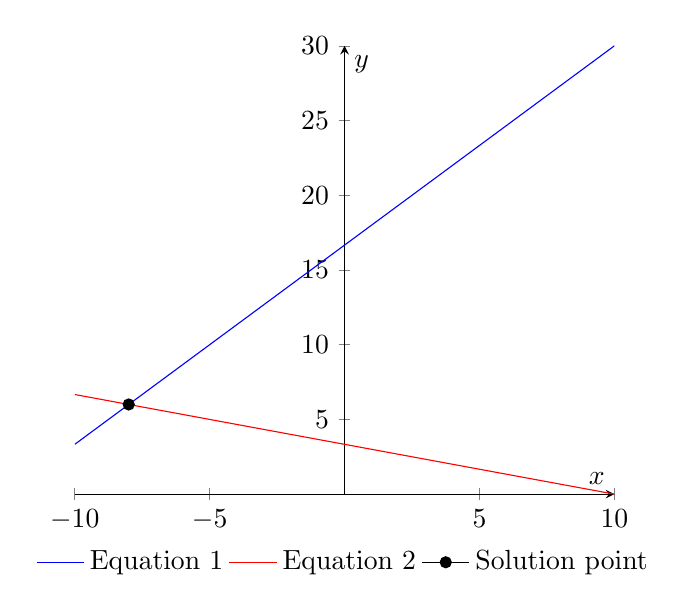
\begin{tikzpicture}
	\begin{axis}[
	xlabel=$x$,
	ylabel=$y$,
	axis lines = center,
	legend style={at={(0.5,-0.1)},anchor=north,draw=none,legend columns=-1}]
	\addplot[domain=-10:10,color=blue]{( 8/ 6)*x-( -100/ 6)};
	\addlegendentry{Equation 1}
	\addplot[domain=-10:10,color=red]{-( 4/ 12)*x+( 40/ 12)};
	\addlegendentry{Equation 2}
	\addplot[mark=*]coordinates {( -8, 6)};
	\addlegendentry{Solution point}
	\end{axis}
	\end{tikzpicture}
	\end{center}
	 \quad \textbf{}
\end{enumerate}\newpage
\end{top_enumerate}
\section{Calculus}
\subsection{Exercise \texttt{Ex\_5}}
source: \texttt{demo/raw\_latex\_exercises/calculus/multivariate\_derivatives.tex}

Randomised parameters in \textbf{bold}. 

\hyperlink{contents}{Back to Table of Contents}
\begin{top_enumerate}
\item A multivariate function is given by:
\[
z = {\bf 10}x^{\bf 6} + {\bf 9}xy + {\bf 10}xy^2 - \frac{x}{y^{\bf 4}}
\]
 
\setcounter{equation}{0}  % reset counter 
\begin{enumerate}
	\setlength{\topsep}{-0pt}
	\setlength{\partopsep}{-0pt}
	\setlength{\itemsep}{10pt}
			\item Find the first-order partial derivative with respect to $x$.
	 \quad \textbf{[2]}
		\item Find the first-order partial derivative with respect to $y$.
	 \quad \textbf{[2]}
		\item Find the second-order partial derivative with respect to $x$.
	 \quad \textbf{[3]}
		\item Find the second-order partial derivative with respect to $y$.
	 \quad \textbf{[3]}
		\item Find the second-order partial derivative with respect to $x$ and $y$.
	 \quad \textbf{[4]}
\end{enumerate}\addtocounter{enumi}{-1}
\item Solutions:
 
\setcounter{equation}{0}  % reset counter 
\begin{enumerate}
	\setlength{\topsep}{-0pt}
	\setlength{\partopsep}{-0pt}
	\setlength{\itemsep}{10pt}
			\item $\frac{\partial z}{\partial x}={{\bf 60}x^{\bf 5} + {\bf 9}y + {\bf 10}y^2 - \frac{1}{y^{\bf 4}}}$
	 \quad \textbf{}
		\item $\frac{\partial z}{\partial y}={{\bf 9}x + {\bf 20}xy + \frac{{\bf 4}x}{y^{\bf 5}}}$
	 \quad \textbf{}
		\item $\frac{\partial^2 z}{\partial x^2}={{\bf 300}x^{\bf 4}}$
	 \quad \textbf{}
		\item $\frac{\partial^2 z}{\partial y^2}={{\bf 20}x - \frac{{\bf 20}x}{y^{\bf 6}}}$
	 \quad \textbf{}
		\item $\frac{\partial^2 z}{\partial x \partial y}={{\bf 9} + {\bf 20}y + \frac{{\bf 4}}{y^{\bf 5}}}$
	 \quad \textbf{}
\end{enumerate}\newpage
\end{top_enumerate}
\subsection{Exercise \texttt{Ex\_6}}
source: \texttt{demo/raw\_latex\_exercises/calculus/total\_derivatives.tex}

Randomised parameters in \textbf{bold}. 

\hyperlink{contents}{Back to Table of Contents}
\begin{top_enumerate}
\item Find the total differentials of the following functions:

(Tip: use 'd' as the total differential operator, so type 'dx' for $\textrm{d}x$)
 
\setcounter{equation}{0}  % reset counter 
\begin{enumerate}
	\setlength{\topsep}{-0pt}
	\setlength{\partopsep}{-0pt}
	\setlength{\itemsep}{10pt}
			\item $f(x,y) = x^{\bf 2} + {\bf 10}x^{\bf 2}y^{\bf 2} + y^{\bf 5}$
	 \quad \textbf{[3]}
		\item $f(x,y) = {\bf 2}x^{\frac{{\bf 8}}{{\bf 9}}}y^{\frac{1}{{\bf 9}}}$
	 \quad \textbf{[3]}
\end{enumerate}\addtocounter{enumi}{-1}
\item The total differential of a function $f(x,y)$ is given by:
\[
\textrm{d}f(x,y) = \frac{\partial f(x,y)}{\partial x}\textrm{d}x + \frac{\partial f(x,y)}{\partial y}\textrm{d}y
\]
 
\setcounter{equation}{0}  % reset counter 
\begin{enumerate}
	\setlength{\topsep}{-0pt}
	\setlength{\partopsep}{-0pt}
	\setlength{\itemsep}{10pt}
			\item The partial derivatives of the function with respect to $x$ and $y$ are:
	\[
	\left\{\begin{aligned}
	\frac{\partial f(x,y)}{\partial x} & = {\bf 2}x + {\bf 20}xy^{\bf 2}\\
	\frac{\partial f(x,y)}{\partial y} & = {\bf 20}x^{\bf 2}y + {\bf 5}y^{\bf 4}\\
	\end{aligned}\right.
	\]
	Replacing in the expression for the total differential gives:
	\[
	\textrm{d}f(x,y) = \left({\bf 2}x + {\bf 20}xy^{\bf 2}\right)\textrm{d}x + \left({\bf 20}x^{\bf 2}y + {\bf 5}y^{\bf 4}\right)\textrm{d}y
	\]
	 \quad \textbf{}
		\item The partial derivatives of the function with respect to $x$ and $y$ are:
	\[
	\left\{\begin{aligned}
	\frac{\partial f(x,y)}{\partial x} & = \frac{{\bf 16}}{{\bf 9}}x^{-\frac{1}{{\bf 9}}}y^{\frac{1}{{\bf 9}}}\\
	\frac{\partial f(x,y)}{\partial y} & = \frac{{\bf 2}}{{\bf 9}}x^{\frac{{\bf 8}}{{\bf 9}}}y^{-\frac{{\bf 8}}{{\bf 9}}}\\
	\end{aligned}\right.
	\]
	Replacing in the expression for the total differential gives:
	\[
	\textrm{d}f(x,y) = \left(\frac{{\bf 16}}{{\bf 9}}x^{-\frac{1}{{\bf 9}}}y^{\frac{1}{{\bf 9}}}\right)\textrm{d}x + \left(\frac{{\bf 2}}{{\bf 9}}x^{\frac{{\bf 8}}{{\bf 9}}}y^{-\frac{{\bf 8}}{{\bf 9}}}\right)\textrm{d}y
	\]
	 \quad \textbf{}
\end{enumerate}\newpage
\end{top_enumerate}
\subsection{Exercise \texttt{Ex\_7}}
source: \texttt{demo/raw\_latex\_exercises/calculus/univariate\_derivatives.tex}

Randomised parameters in \textbf{bold}. 

\hyperlink{contents}{Back to Table of Contents}
\begin{top_enumerate}
\item Differentiate each of the following functions with respect to $x$. Use an appropriate notation in each case.
 
\setcounter{equation}{0}  % reset counter 
\begin{multicols}{2}
\begin{enumerate}
	\setlength{\topsep}{-0pt}
	\setlength{\partopsep}{-0pt}
	\setlength{\itemsep}{10pt}
			\item $y = {\bf -12}$
	 \quad \textbf{[1]}
		\item $y = {\bf 25}$
	 \quad \textbf{[1]}
		\item $y = {\bf -13}x+{\bf 8}$
	 \quad \textbf{[1]}
		\item $f(x) = {\bf -11}x-{\bf 8}$
	 \quad \textbf{[1]}
		\item $y = {\bf 4}x^2$
	 \quad \textbf{[2]}
		\item $f(x)={\bf -3}x^{\bf 4}$
	 \quad \textbf{[2]}
		\item $y = {\bf 10}x^3 - {\bf 3}x^2 + {\bf 6}x + {\bf 10}$
	 \quad \textbf{[2]}
		\item $y = {\bf 6}x^{\bf 8} + {\bf 3}x^{\bf 5} - {\bf 10}x^{\bf 2} - {\bf 10}$
	 \quad \textbf{[2]}
\end{enumerate}\end{multicols}\addtocounter{enumi}{-1}
\item Solutions:
 
\setcounter{equation}{0}  % reset counter 
\begin{multicols}{2}
\begin{enumerate}
	\setlength{\topsep}{-0pt}
	\setlength{\partopsep}{-0pt}
	\setlength{\itemsep}{10pt}
			\item $\frac{\textrm{d}y}{\textrm{d}x}={{\bf 0}}$
	 \quad \textbf{}
		\item $\frac{\textrm{d}}{\textrm{d}x}y={{\bf 0}}$
	 \quad \textbf{}
		\item $y'={{\bf -13}}$
	 \quad \textbf{}
		\item $f'(x)={{\bf -11}}$
	 \quad \textbf{}
		\item $\frac{\textrm{d}}{\textrm{d}x}({\bf 4}x^2)={{\bf 8}x}$
	 \quad \textbf{}
		\item $f_x={{\bf -12}x^{\bf 3}}$
	 \quad \textbf{}
		\item $\frac{\textrm{d}y}{\textrm{d}x}={{\bf 30}x^2 - {\bf 6}x + {\bf 6}}$
	 \quad \textbf{}
		\item $\frac{\textrm{d}y}{\textrm{d}x}={{\bf 48}x^{\bf 7} + {\bf 15}x^{\bf 4} - {\bf 20}x}$
	 \quad \textbf{}
\end{enumerate}\end{multicols}\newpage
\end{top_enumerate}
\chapter{Statistics}
\section{Inference}
\subsection{Exercise \texttt{Ex\_10}}
source: \texttt{demo/raw\_latex\_exercises/statistics/confidence\_large.tex}

Randomised parameters in \textbf{bold}. 

\hyperlink{contents}{Back to Table of Contents}
\begin{top_enumerate}
\item A random sample of size $n={\bf 58}$ is taken from a large population with known standard deviation $\sigma = {\bf 32}$. If the sample mean is {\bf 79}, calculate to 2 decimal places the following confidence intervals for the population mean $\mu$:
 
\setcounter{equation}{0}  % reset counter 
\begin{enumerate}
	\setlength{\topsep}{-0pt}
	\setlength{\partopsep}{-0pt}
	\setlength{\itemsep}{10pt}
			\item The 90\% confidence interval.
	 \quad \textbf{[3]}
		\item The 95\% confidence interval.
	 \quad \textbf{[3]}
		\item The 99\% confidence interval.
	 \quad \textbf{[3]}
\end{enumerate}\addtocounter{enumi}{-1}
\item Solution:
 
\setcounter{equation}{0}  % reset counter 
\begin{enumerate}
	\setlength{\topsep}{-0pt}
	\setlength{\partopsep}{-0pt}
	\setlength{\itemsep}{10pt}
			\item If the sample of size $n={\bf 58}$ has a mean $\bar x = {\bf 79}$ and the population has a standard deviation $\sigma={\bf 32}$, then the sampling distribution of the mean follows a normal distribution:
	\[
	\bar X \sim N \left(\bar x,\frac{\sigma^2}{n}\right) = N \left({\bf 79},\frac{{\bf 32}^2}{{\bf 58}}\right) = N \left({\bf 79},{\bf 17.66}\right)
	\]
	Note, we are given the population standard deviation $\sigma$, which means that we can use the Normal distribution to calculate the confidence interval regardless of sample size (i.e. we do not need the Central Limit Theorem).
	
	The 90\% confidence interval can be constructed using the standard normal distribution, but looking for the value of $z$ such that:
	\[
	P(-z < Z < z) = 0.9 \quad \iff \quad P(0 \le Z \le z) = 0.45
	\]
	Using the table of values, we find $z = \pm 1.645$. Using the mean and standard deviation of the distribution of $\bar X$, we can then recover 90\% confidence interval.
	\[
	C.I._{90} = \bar x \pm 1.645 \frac{\sigma}{\sqrt{n}} = {\bf 79} \pm 1.645 \cdot {\bf 4.20} = ({\bf 72.09}, {\bf 85.91})
	\]
	With 90\% confidence, the population mean $\mu$ is between {\bf 72.09} and {\bf 85.91}.
	 \quad \textbf{}
		\item The 95\% confidence interval can be constructed by looking for the value of $z$ such that:
	\[
	P(-z < Z < z) = 0.95 \quad \iff \quad P(0 \le Z \le z) = 0.475
	\]
	Using the table of values, we find $z = \pm 1.96$. Using the mean and standard deviation of the distribution of $\bar X$, we can then recover 95\% confidence interval.
	\[
	C.I._{95} = \bar x \pm 1.96 \frac{\sigma}{\sqrt{n}} = {\bf 79} \pm 1.96 \cdot {\bf 4.20} = ({\bf 70.77}, {\bf 87.23})
	\]
	With 95\% confidence, the population mean $\mu$ is between {\bf 70.77} and {\bf 87.23}.
	 \quad \textbf{}
		\item The 99\% confidence interval can be constructed by looking for the value of $z$ such that:
	\[
	P(-z < Z < z) = 0.99 \quad \iff \quad P(0 \le Z \le z) = 0.495
	\]
	Using the table of values, we find $z = \pm 2.575$. Using the mean and standard deviation of the distribution of $\bar X$, we can then recover 99\% confidence interval.
	\[
	C.I._{99} = \bar x \pm 2.575 \frac{\sigma}{\sqrt{n}} = {\bf 79} \pm 2.575 \cdot {\bf 4.20} = ({\bf 68.19}, {\bf 89.81})
	\]
	With 99\% confidence, the population mean $\mu$ is between {\bf 68.19} and {\bf 89.81}.
	 \quad \textbf{}
\end{enumerate}\newpage
\end{top_enumerate}
\subsection{Exercise \texttt{Ex\_11}}
source: \texttt{demo/raw\_latex\_exercises/statistics/confidence\_small.tex}

Randomised parameters in \textbf{bold}. 

\hyperlink{contents}{Back to Table of Contents}
\begin{top_enumerate}
\item A random sample of size $n={\bf 9}$ is taken from a large population. The sample mean is $\bar x = {\bf 89}$, and the sample standard deviation is $s = {\bf 31}$.
 
\setcounter{equation}{0}  % reset counter 
\begin{enumerate}
	\setlength{\topsep}{-0pt}
	\setlength{\partopsep}{-0pt}
	\setlength{\itemsep}{10pt}
			\item Using this information, construct a 95\% confidence interval for the population mean $\mu$. Enter the interval using square brackets, separating the two values with commas $\left[\dots ,\dots \right]$:
	 \quad \textbf{[2]}
		\item Suppose you are told that {\bf 31} is also the value of the population standard deviation $\sigma$. Construct a new 95\% confidence interval and compare this with your previous calculation.
	 \quad \textbf{[3]}
\end{enumerate}\addtocounter{enumi}{-1}
\item Solution:
 
\setcounter{equation}{0}  % reset counter 
\begin{enumerate}
	\setlength{\topsep}{-0pt}
	\setlength{\partopsep}{-0pt}
	\setlength{\itemsep}{10pt}
			\item Given that the sample has a size $n={\bf 9}$, if we do not know the population standard deviation $\sigma$, then we need to (a) replace $\sigma$ by the sample standard deviation $s$ and (b) rely on the $t$-distribution instead of the standard normal distribution, to allow for additional uncertainty generated by using $s$, which is an estimate of $\sigma$:
	\[
	C.I._{95} = \bar x \pm t_{0.05}^{n-1} \frac{s}{\sqrt{n}}
	\]
	
	The critical value $t_{0.05}^{n-1}$ can be found in the table of values for Student's t-distribution, for a two-tailed probability of 0.05 (corresponding to 95\% confidence) and $n-1 = {{\bf 9}-1}$ degrees of freedom. In this case, $t_{0.05}^{{\bf 9}-1} = {\bf 2.306}$. This gives us the following confidence interval:
	\[
	C.I._{95} =  {\bf 89} \pm {\bf 2.306}\frac{{\bf 31}}{\sqrt{{\bf 9}}}  =  \left[{\bf 65.17} \, , \, {\bf 112.83}\right]
	\]
	 \quad \textbf{}
		\item If the sample of size $n={\bf 9}$ has a mean $\bar x = {\bf 89}$ and the population has standard deviation $\sigma={\bf 31}$, then the sampling distribution of the mean follows a normal distribution:
	\[
	\bar X \sim N \left(\bar x,\frac{\sigma^2}{n}\right) = N \left({\bf 89},\frac{{\bf 31}^2}{{\bf 9}}\right) \approx N \left({\bf 89},{\bf 10.333}^2\right)
	\]
	Note, because we now know the value of the population standard deviation $\sigma$, we are able to calculate confidence intervals using the normal distribution, and we do not need to use Student's t-distribution. This is only required when (a) we use the sample standard deviation $s$ as an estimate of $\sigma$ and (b) the sample size $n<30$, so that there is a lot of uncertainty in the accuracy of $s$.
	
	The 95\% confidence interval can be constructed using the standard normal distribution, but looking for the value of $z$ such that:
	\[
	P(-z < Z < z) = 0.95 \quad \iff \quad P(0 \le Z \le z) = 0.475
	\]
	Using the table of values, we find $z = \pm 1.96$. Using the mean and standard deviation of the distribution of $\bar X$, we can then calculate 95\% confidence interval.
	\[
	C.I._{95} = \bar x \pm 1.96 \frac{\sigma}{\sqrt{n}} = {\bf 89} \pm 1.96 \frac{{\bf 31}}{\sqrt{{\bf 9}}} = \left[{\bf 68.75} \, , \, {\bf 109.25}\right]
	\]
	This is much tighter confidence interval than the previous answer. Even if the actual value of the standard deviation has not changed (still $p3$), the fact that we know for certain the value of the population standard deviation $\sigma$ rather than have to rely on an estimate $s$ means we can be much more precise for a given confidence level.
	 \quad \textbf{}
\end{enumerate}\newpage
\end{top_enumerate}
\subsection{Exercise \texttt{Ex\_13}}
source: \texttt{demo/raw\_latex\_exercises/statistics/hypothesis.tex}

Randomised parameters in \textbf{bold}. 

\hyperlink{contents}{Back to Table of Contents}
\begin{top_enumerate}
\item A pair of dice is tossed {\bf 100} times and the sum is seven {\bf 28} times.
 
\setcounter{equation}{0}  % reset counter 
\begin{enumerate}
	\setlength{\topsep}{-0pt}
	\setlength{\partopsep}{-0pt}
	\setlength{\itemsep}{10pt}
			\item If the dice were fair, what would be the probability of the sum being seven? Round to 3 decimal places if required.
	 \quad \textbf{[3]}
		\item We can reject the hypothesis that the dice are fair using a two tailed test at 5\% significance. True or False?
	 \quad \textbf{[3]}
		\item We can reject the hypothesis that the dice are fair using a one tailed test at 5\% significance. True or False? Explain which type of test you think is more appropriate in this case.
	 \quad \textbf{[3]}
\end{enumerate}\addtocounter{enumi}{-1}
\item Solution:
 
\setcounter{equation}{0}  % reset counter 
\begin{enumerate}
	\setlength{\topsep}{-0pt}
	\setlength{\partopsep}{-0pt}
	\setlength{\itemsep}{10pt}
			\item With two dice, a throw will result in $6^2=36$ possible pairs of faces. There are $6$ possible ways that the sum of the two faces $X$ can be $7$:
	\[
	\begin{aligned}
	1 + 6 \quad & \quad 2 + 5 \quad & \quad 3 + 4\\
	4 + 3 \quad & \quad 5 + 2 \quad & \quad 6 + 1\\
	\end{aligned}
	\]
	If the dice are fair, all 36 outcomes are equally probable and the probability is therefore:
	$P\left(X = 7 \right) = \frac{6}{36} = \frac{1}{6}$
	 \quad \textbf{}
		\item The information required to set up the hypothesis test is that the true proportion is $p = \frac{1}{6}$, while the sample proportion is $\hat p = {\bf 0.28}$ with a population standard deviation component $\sigma = \sqrt{\frac{6}{36} \times \frac{30}{36}} = \sqrt{\frac{5}{36}}$ (remember, we assume that the null is true!). The sample size is $n={\bf 100}$, therefore we can draw the critical values from the normal distribution.
	
	The hypotheses we want to test are:
	\[
	\left\{\begin{aligned}
	H_0: \, & p = \frac{1}{6} \\
	H_1: \, & p \ne \frac{1}{6} \\
	\end{aligned}\right.
	\]
	
	The test statistic is:
	\[
	t = \frac{\hat p - p}{\frac{\sigma}{\sqrt{n}}} = \frac{{\bf 0.28}-\frac{1}{6}}{\sqrt{\frac{5}{36\times{\bf 100}}}} = \frac{{\bf 0.113}}{{\bf 0.037}} = {\bf 3.041}
	\]
	
	Given that we want 95\% confidence on a two-tailed test with a sample size of $n={\bf 100}$, the critical value of the t-statistic is $z_{0.05} = 1.96$. This tells us that $t < z_{0.02}$, therefore there is {\bf   }enough evidence to reject the null hypothesis that the dice are fair. The statement is \emph{{\bf true}}.
	 \quad \textbf{}
		\item For the one-tailed test, given that $\hat p > p$, we can set up the following hypotheses:
	\[
	\left\{\begin{aligned}
	H_0: \, & p \le \frac{1}{6} \\
	H_1: \, & p > \frac{1}{6} \\
	\end{aligned}\right.
	\]
	
	The  test statistic is the same as before, $t = {\bf 3.041}$ If we want 95\% confidence, on a one-tailed test the critical value of the t-statistic becomes $z_{0.1} = 1.645$. This tells us that $t > z_{0.1}$, therefore we {\bf  can  }reject the null hypothesis that the dice are fair. The statement is \emph{{\bf true}}.
	
	The difference here rests in the choice of alternate hypothesis. In a two-tailed test, the alternate hypothesis is $H_1: \, p \ne \frac{1}{6}$. We are simply stating the sample proportion is not equal to the stated proportion: it could be higher, or it could be lower. In the absence of information about how the dice might be unfair, this is the most conservative approach as it allows for either possibility. In contrast, with the one-tailed test, we have $H_1: \, p > \frac{1}{6}$: we are explicitly ruling out the possibility that the true proportion is lower than {\bf 16.667} out of {\bf 100}. This assumption allows us to reject the null more easily (i.e. with a smaller deviation from the stated proportion), at the risk of being very wrong if our assumption was incorrect.
	
	\begin{center}
	\begin{tikzpicture}
	\begin{axis}[
	    samples = 50,
	    axis lines = center,
	    legend style={at={(0.5,-0.1)},anchor=north, draw=none},
	    ymin=0,
	    ymax=0.75,
	    xmin=-4,
	    xmax=4,
	    xlabel = $x$,
	    ylabel = $f(x)$
	]
	\addplot[domain=-4:4,color=blue,]{0.39894228*exp(-0.5*x^2)};
	\addlegendentry{$N(0,1)$}
	\addplot[mark=no,color=black] coordinates { ( 3.041, 0) ( 3.041, 0.5)};
	\addlegendentry{$t$}
	\addplot[mark=no,color=red] coordinates { (1.96, 0) (1.96, 0.5)};
	\addlegendentry{$z_{0.05} = 1.96$}
	\addplot[mark=no,dashed,color=green] coordinates { (1.645, 0) (1.645, 0.5)};
	\addlegendentry{$z_{0.1} = 1.645$}
	\end{axis}
	\end{tikzpicture}
	\end{center}
	 \quad \textbf{}
\end{enumerate}\newpage
\end{top_enumerate}
\subsection{Exercise \texttt{Ex\_17}}
source: \texttt{demo/raw\_latex\_exercises/statistics/sample\_size.tex}

Randomised parameters in \textbf{bold}. 

\hyperlink{contents}{Back to Table of Contents}
\begin{top_enumerate}
\item You are told that a random variable $X$ has a population standard deviation of {\bf 9}.
 
\setcounter{equation}{0}  % reset counter 
\begin{enumerate}
	\setlength{\topsep}{-0pt}
	\setlength{\partopsep}{-0pt}
	\setlength{\itemsep}{10pt}
			\item How large a sample $n$ would you need in order to be able to estimate the population mean to within $\pm${\bf 1.5} at the {\bf 90}\% confidence level? Round your answer up to an integer.
	 \quad \textbf{[2]}
\end{enumerate}\addtocounter{enumi}{-1}
\item Solution:
 
\setcounter{equation}{0}  % reset counter 
\begin{enumerate}
	\setlength{\topsep}{-0pt}
	\setlength{\partopsep}{-0pt}
	\setlength{\itemsep}{10pt}
			\item In order to determine how large a sample we need to achieve an error of $\pm${\bf 1.5} at {\bf 90}\% confidence, we can invert the formula for the confidence interval, where $z_{{\bf 90}}$ is the critical value of the standard normal distribution. Suppose we pick the upper $U_{{\bf 90}}$ bound of the confidence interval:
	
	\[
	\begin{aligned}
	U_{{\bf 90}} & = \bar x + z_{{\bf 90}} \frac{\sigma}{\sqrt{n}}\\
	U_{{\bf 90}} - \bar x  & = z_{{\bf 90}} \frac{\sigma}{\sqrt{n}}\\
	\sqrt{n} & =z_{{\bf 90}} \frac{\sigma}{U_{{\bf 90}} - \bar x} \\
	n & = \left(z_{{\bf 90}} \frac{\sigma}{U_{{\bf 90}} - \bar x}\right)^2 \\
	\end{aligned}
	\]
	
	The {\bf 90}\% critical value interval can be constructed using the standard normal distribution, but looking for the value of $z_{{\bf 90}}$ such that:
	\[
	P(-z_{{\bf 90}} < Z < z_{{\bf 90}}) = {\bf 0.9} \quad \iff \quad P(0 \le Z \le z_{{\bf 90}}) = {\bf 0.45}
	\]
	Using the table of values, we find $z_{{\bf 90}} = {\bf 1.645}$. Replacing this in the equation above, and including the information that the upper bound of the confidence interval should be {\bf 1.5} above the mean, we can find the required sample size.
	
	\[
	n = \left({\bf 1.645} \frac{{\bf 9}}{{\bf 1.5}}\right)^2 \approx \left({\bf 9.87}\right)^2 \approx {\bf 97.417}
	\]
	We need a sample of at least {\bf 98} observations in order to generate a confidence interval of $\pm${\bf 1.5} around the sample mean.
	 \quad \textbf{}
\end{enumerate}\newpage
\end{top_enumerate}
\section{Probability and descriptive stats}
\subsection{Exercise \texttt{Ex\_12}}
source: \texttt{demo/raw\_latex\_exercises/statistics/descriptive.tex}

Randomised parameters in \textbf{bold}. 

\hyperlink{contents}{Back to Table of Contents}
\begin{top_enumerate}
\item A sample of 100 UK households have the following distribution:

\begin{center}
\begin{tabular}{cc}
Household size & Frequency $f_i$ \\
\hline
1 & {\bf 24} \\
2 & {\bf 31} \\
3 & {\bf 15} \\
4 & {\bf 19} \\
5 & {\bf 7} \\
6 & {\bf 4} \\
\hline
\end{tabular}
\end{center}
 
\setcounter{equation}{0}  % reset counter 
\begin{enumerate}
	\setlength{\topsep}{-0pt}
	\setlength{\partopsep}{-0pt}
	\setlength{\itemsep}{10pt}
			\item Calculate the mean household size $\bar x$. Round your answer to two decimal places if needed.
	 \quad \textbf{[3]}
		\item Calculate the median household size $\tilde x$.
	 \quad \textbf{[2]}
		\item Calculate the mode.
	 \quad \textbf{[2]}
		\item Calculate the sample standard deviation $s$, rounded to 2 decimal places.
	 \quad \textbf{[3]}
\end{enumerate}\addtocounter{enumi}{-1}
\item Solutions:
 
\setcounter{equation}{0}  % reset counter 
\begin{enumerate}
	\setlength{\topsep}{-0pt}
	\setlength{\partopsep}{-0pt}
	\setlength{\itemsep}{10pt}
			\item The frequency table is given by:
	
	\begin{center}
	\begin{tabular}{cccc}
	Household size & Frequency $f_i$ & $f_i x_i$ & $f_i (x_i-\bar x)^2$\\
	\hline
	1 & {\bf 24} & {\bf 24} & {\bf 66.13}\\
	2 & {\bf 31} & {\bf 62} & {\bf 13.50}\\
	3 & {\bf 15} & {\bf 45} & {\bf 1.73}\\
	4 & {\bf 19} & {\bf 76} & {\bf 34.12}\\
	5 & {\bf 7} & {\bf 35} & {\bf 38.33}\\
	6 & {\bf 4} & {\bf 24} & {\bf 44.62}\\
	\hline
	Total & 100 & {\bf 266} & {\bf 198.44} \\
	\hline
	\end{tabular}
	\end{center}
	
	\[
	\bar x = \frac{\sum_i f_i x_i}{N} =\frac{\bf 266}{100} = {\bf 2.66}
	\]
	 \quad \textbf{}
		\item \[
	\tilde x = {\bf 2}
	\]
	 \quad \textbf{}
		\item \[
	\textrm{Mode} = {\bf 2}
	\]
	 \quad \textbf{}
		\item \[
	s^2 = \frac{\sum_i f_i (x_i-\bar x)^2}{N-1} =\frac{{\bf 198.44}}{99} \approx {\bf 2.00}
	\]
	If the sample variance is $s^2 \approx {\bf 2.00}$ then the sample standard deviation is $s \approx \sqrt{{\bf 2.00}} \approx {\bf 1.42}$
	 \quad \textbf{}
\end{enumerate}\newpage
\end{top_enumerate}
\subsection{Exercise \texttt{Ex\_16}}
source: \texttt{demo/raw\_latex\_exercises/statistics/probabilities.tex}

Randomised parameters in \textbf{bold}. 

\hyperlink{contents}{Back to Table of Contents}
\begin{top_enumerate}
\item You are told $P(A) = {\bf 0.26}$, $P(B) = {\bf 0.66}$ and $P(A \textrm{ or } B) = {\bf 0.85}$. Are the following statements true or false? Provide an explanation in each case.
 
\setcounter{equation}{0}  % reset counter 
\begin{enumerate}
	\setlength{\topsep}{-0pt}
	\setlength{\partopsep}{-0pt}
	\setlength{\itemsep}{10pt}
			\item $A$ and $B$ are independent.
	 \quad \textbf{[3]}
		\item $A$ and $B$ are mutually exclusive.
	 \quad \textbf{[3]}
		\item If two events that occur with non-zero probabilities are mutually exclusive, then they cannot be independent.
	 \quad \textbf{[4]}
\end{enumerate}\addtocounter{enumi}{-1}
\item Solutions:
 
\setcounter{equation}{0}  % reset counter 
\begin{enumerate}
	\setlength{\topsep}{-0pt}
	\setlength{\partopsep}{-0pt}
	\setlength{\itemsep}{10pt}
			\item By the addition rule we know that $P(A \textrm{ and } B) = P(A) + P(B) - P(A \textrm{ or } B)$. Using the values above, this give us:
	\[
	P(A \textrm{ and } B) = {\bf 0.26} + {\bf 0.66} - {\bf 0.85} = {\bf 0.07}
	\]
	Furthermore, we can calculate:
	\[
	P(A)\times P(B) = {\bf 0.26} \times {\bf 0.66} = {\bf 0.17}
	\]
	Because $P(A \textrm{ and } B) \, {\bf  \ne} \, P(A)\times P(B)$, one can conclude that $A$ and $B$ are {\bf  not }independent. \emph{{\bf false}}
	 \quad \textbf{}
		\item $A$ and $B$ cannot be mutually exclusive, as $P(A \textrm{ and } B) = {\bf 0.07} \ne 0$. There is a probability that both events will happen together. \emph{False}
	 \quad \textbf{}
		\item If two events $A$ and $B$ are mutually exclusive, then $P(A \textrm{ and } B) = 0$. If these two events are also independent, then  we also have $P(A \textrm{ and } B) = P(A)\times P(B)$. The combination of the two implies:
	\[
	P(A \textrm{ and } B) = P(A)\times P(B) = 0
	\]
	This can only be the case if at least one of the events has a zero probability. As we are told that both events have non-zero probability, they cannot be mutually exclusive and independent. \emph{True}.
	 \quad \textbf{}
\end{enumerate}\newpage
\end{top_enumerate}
\subsection{Exercise \texttt{Ex\_18}}
source: \texttt{demo/raw\_latex\_exercises/statistics/urns\_balls.tex}

Randomised parameters in \textbf{bold}. 

\hyperlink{contents}{Back to Table of Contents}
\begin{top_enumerate}
\item A ball is drawn from a box containing {\bf 8} red, {\bf 28} white, {\bf 18} blue and {\bf 14} orange balls. Find the probability (rounded to 2 decimal places if required) that it is:
 
\setcounter{equation}{0}  % reset counter 
\begin{enumerate}
	\setlength{\topsep}{-0pt}
	\setlength{\partopsep}{-0pt}
	\setlength{\itemsep}{10pt}
			\item Orange or red.
	 \quad \textbf{[1]}
		\item Not red and not blue.
	 \quad \textbf{[1]}
		\item Not blue.
	 \quad \textbf{[1]}
		\item White.
	 \quad \textbf{[1]}
\end{enumerate}\addtocounter{enumi}{-1}
\item Solutions:
 
\setcounter{equation}{0}  % reset counter 
\begin{enumerate}
	\setlength{\topsep}{-0pt}
	\setlength{\partopsep}{-0pt}
	\setlength{\itemsep}{10pt}
			\item There are ${\bf 8} + {\bf 28} + {\bf 18} + {\bf 14} = {\bf 68}$ balls in total in the box. The probabilities can be calculated by counting the number of balls that meet the condition described in the event and dividing by the total number of balls (${\bf 68}$). In this case we are using $P(O \textrm{ or } R) = P(O) + P(R)$, as the draw is mutually exclusive: we cannot draw both an orange and a red, so $P(O \textrm{ and } R) = 0$.
	\[
	P(O \textrm{ or } R) = \frac{{\bf 14} + {\bf 8}}{\bf 68} \approx {\bf 0.32}
	\]
	 \quad \textbf{}
		\item The most direct route is to realise that the only types of balls that are simultaneously `not red' and `not blue' are the orange and white ones, which directly gives:
	
	\[
	P(\textrm{not } R \textrm{ and not } B) =  P( O \textrm{and } W) = \frac{{\bf 14}+{\bf 28}}{{\bf 68}} = \frac{{\bf 42}}{{\bf 68}} \approx {\bf 0.62}
	\]
	
	Alternatively, you can also work out the solution using the addition rule. This takes a bit longer and the use of `not' can complicate thinking about this, but the formula still works:
	
	\[
	P(\textrm{not } R \textrm{ or not } B) = P(\textrm{not } R) + P(\textrm{not } B) - P(\textrm{not } R \textrm{ and not } B)
	\]
	
	Rearranging:
	
	\[
	P(\textrm{not } R \textrm{ and not } B) = P(\textrm{not } R) + P(\textrm{not } B) - P(\textrm{not } R \textrm{ or not } B)
	\]
	
	A key aspect is to realise that $P(\textrm{not } R \textrm{ or not } B) = 1$. Any ball you pick is guaranteed to be either `not red' or `not blue'. This is obviously true for the orange and white balls, but also the red and blue ones: a red ball is `not blue' and a blue ball is `not red'! Using this, and replacing $P(\textrm{not } R) = 1 - P(R)$ and $P(\textrm{not } B) = 1 - P(B)$ we get:
	
	\[
	P(\textrm{not } R \textrm{ and not } B) = 1 - P(R) + 1 - P(B) - 1 \; = \; 1 - P(R) - P(B)
	\]
	
	\[
	P(\textrm{not } R \textrm{ and not } B) = \frac{{\bf 68} - {\bf 8} - {\bf 18}}{{\bf 68}} = \frac{{\bf 42}}{{\bf 68}}
	\]
	 \quad \textbf{}
		\item \[
	P(\textrm{not } B) = 1 - P(B) = \frac{{\bf 68} - {\bf 18}}{{\bf 68}} = \frac{{\bf 50}}{{\bf 68}} \approx {\bf 0.74}
	\]
	 \quad \textbf{}
		\item \[
	P(W) = \frac{\bf 28}{\bf 68} \approx {\bf 0.41}
	\]
	 \quad \textbf{}
\end{enumerate}\newpage
\end{top_enumerate}
\section{Probability distributions}
\subsection{Exercise \texttt{Ex\_8}}
source: \texttt{demo/raw\_latex\_exercises/statistics/binomial\_1.tex}

Randomised parameters in \textbf{bold}. 

\hyperlink{contents}{Back to Table of Contents}
\begin{top_enumerate}
\item Suppose {\bf 22}\% of customers at Aldi pay by cash. In a random sample of {\bf 13} customers, what is the probability (rounded to 4 decimal places) that:
 
\setcounter{equation}{0}  % reset counter 
\begin{enumerate}
	\setlength{\topsep}{-0pt}
	\setlength{\partopsep}{-0pt}
	\setlength{\itemsep}{10pt}
			\item Two of the customers pay by cash?
	 \quad \textbf{[2]}
		\item At least two of the customers pay by cash?
	 \quad \textbf{[2]}
\end{enumerate}\addtocounter{enumi}{-1}
\item Solutions:

The probability of a given number of customers $X$ paying in cash can be modelled using a Binomial distribution, with $N={\bf 13}$ being the number of trials and $p={\bf 0.22}$ the probability of a success (paying in cash):
\[
P(X=k \, | \, n={\bf 13},p={\bf 0.22}) \quad = \quad C^{{\bf 13}}_k {\bf 0.22}^k {\bf 0.78}^{{\bf 13}-k}
\]
 
\setcounter{equation}{0}  % reset counter 
\begin{enumerate}
	\setlength{\topsep}{-0pt}
	\setlength{\partopsep}{-0pt}
	\setlength{\itemsep}{10pt}
			\item \[
	P(X = 2)  = C^{{\bf 13}}_2 {\bf 0.22}^2 {\bf 0.78}^{{\bf 13}-2} \approx {\bf 0.2455}
	\]
	 \quad \textbf{}
		\item To calculated $P(X \ge 2)$, one first decomposes the probability as:
	\[
	P(X \ge 2) = 1 - P(X<2) = 1 - P(X=0) - P(X=1)
	\]
	Each individual probability can be calculated using the binomial formula:
	\[
	\begin{aligned}
	P(X \ge 2) &= 1 - C^{{\bf 13}}_0 {\bf 0.22}^0 {\bf 0.78}^{{\bf 13}} - C^{{\bf 13}}_1 {\bf 0.22}^1 {\bf 0.78}^{{\bf 13}-1}\\
	P(X \ge 2) &\approx 1 - {\bf 0.0396} - {\bf 0.1450} \\
	P(X \ge 2) &\approx {\bf 0.8154} \\
	\end{aligned}
	\]
	 \quad \textbf{}
\end{enumerate}\newpage
\end{top_enumerate}
\subsection{Exercise \texttt{Ex\_9}}
source: \texttt{demo/raw\_latex\_exercises/statistics/binomial\_2.tex}

Randomised parameters in \textbf{bold}. 

\hyperlink{contents}{Back to Table of Contents}
\begin{top_enumerate}
\item What is the probability, rounded to 4 decimal places:
 
\setcounter{equation}{0}  % reset counter 
\begin{enumerate}
	\setlength{\topsep}{-0pt}
	\setlength{\partopsep}{-0pt}
	\setlength{\itemsep}{10pt}
			\item Of getting exactly {\bf 6} heads and {\bf 3} tails in {\bf 9} tosses of a fair coin?
	 \quad \textbf{[3]}
		\item Of getting {\bf 2} sixes in {\bf 9} rolls of a fair dice?
	 \quad \textbf{[3]}
\end{enumerate}\addtocounter{enumi}{-1}
\item Solutions:
 
\setcounter{equation}{0}  % reset counter 
\begin{enumerate}
	\setlength{\topsep}{-0pt}
	\setlength{\partopsep}{-0pt}
	\setlength{\itemsep}{10pt}
			\item The probability of getting $H$ heads can be calculated using a Binomial distribution, with $N={\bf 9}$ being the number of trials and $p=1/2$ being the probability of a success (getting a heads):
	\[
	P(H = {\bf 6})  = C^{{\bf 9}}_{{\bf 6}}  \left(\frac{1}{2}\right)^{{\bf 9}} \approx {\bf 0.1641}
	\]
	Note that we define $H$ as the number of heads, however one could chose instead to count the number of tails. The binomial formula should provide the same answers in both cases, as $C^{{\bf 9}}_{{\bf 6}} = C^{{\bf 9}}_{{\bf 3}}$ and $p=1-p=1/2$. Hopefully this is intuitive, the probability of the event should be the same whether you count heads or tails.
	 \quad \textbf{}
		\item The probability of getting $X$ sixes can be calculated using a Binomial distribution, with $N={\bf 9}$ being the number of trials and $p=1/6$ being the probability of a success (getting a six):
	\[
	P(X = {\bf 2})  = C^{{\bf 9}}_{{\bf 2}}  \left(\frac{1}{6}\right)^{{\bf 2}} \left(\frac{5}{6}\right)^{{\bf 7}} \approx {\bf 0.2791}
	\]
	 \quad \textbf{}
\end{enumerate}\newpage
\end{top_enumerate}
\subsection{Exercise \texttt{Ex\_14}}
source: \texttt{demo/raw\_latex\_exercises/statistics/normal\_crit.tex}

Randomised parameters in \textbf{bold}. 

\hyperlink{contents}{Back to Table of Contents}
\begin{top_enumerate}
\item If $Z \sim N(0,1)$, find the critical value $z_0$, rounded to 2 decimal places, such that:
 
\setcounter{equation}{0}  % reset counter 
\begin{enumerate}
	\setlength{\topsep}{-0pt}
	\setlength{\partopsep}{-0pt}
	\setlength{\itemsep}{10pt}
			\item $P(Z \ge z_0) = {\bf 0.09}$
	 \quad \textbf{[2]}
		\item $P(Z \le z_0) = {\bf 0.27}$
	 \quad \textbf{[2]}
		\item $P(-z_0 \le Z \le z_0) = {\bf 0.46}$
	 \quad \textbf{[2]}
\end{enumerate}\addtocounter{enumi}{-1}
\item Solutions:

Note: It may help you to draw pictures to visualise the area you are being asked to calculate.
 
\setcounter{equation}{0}  % reset counter 
\begin{enumerate}
	\setlength{\topsep}{-0pt}
	\setlength{\partopsep}{-0pt}
	\setlength{\itemsep}{10pt}
			\item If $P(Z \ge z_0) = {\bf 0.09}$, then $P(0 \le Z \le z_0)  = 0.5 - P(z \ge z_0) = {\bf 0.41}$. Looking this value up in the table for the standard normal tells us that $z_0 = {\bf 1.341}$.
	 \quad \textbf{}
		\item If $P(Z \le z_0) = {\bf 0.27}$, then $P(z_0 \le z \le 0) = 0.5 - P(Z \le z_0) = {\bf 0.23}$. In the tables of the standard distribution, this corresponds to a value of ${\bf 0.613}$. However, we are looking for a value of $z$ that is smaller than $z_0$, therefore to the left of it. Given that the probability is less than 0.5, the critical value $z_0$ must be negative. We therefore have $z_0 = -{\bf 0.613}$. A diagram can be particularly useful for cases like this.
	 \quad \textbf{}
		\item If $P(-z_0 \le Z \le z_0) = {\bf 0.46}$ then $P(0 \le Z \le z_0) = \frac{{\bf 0.46}}{2} = {\bf 0.23}$. Looking up this value in the table tells us that $z_0 = {\bf 0.613}$.
	 \quad \textbf{}
\end{enumerate}\newpage
\end{top_enumerate}
\subsection{Exercise \texttt{Ex\_15}}
source: \texttt{demo/raw\_latex\_exercises/statistics/normal\_prob.tex}

Randomised parameters in \textbf{bold}. 

\hyperlink{contents}{Back to Table of Contents}
\begin{top_enumerate}
\item Using the table of areas for the standard Normal distribution, calculate the areas under $N(0,1)$, rounded to 3 decimal places:
 
\setcounter{equation}{0}  % reset counter 
\begin{enumerate}
	\setlength{\topsep}{-0pt}
	\setlength{\partopsep}{-0pt}
	\setlength{\itemsep}{10pt}
			\item Between {\bf -2.575} and {\bf 2.575}
	 \quad \textbf{[2]}
		\item For values greater than {\bf 2.575}
	 \quad \textbf{[2]}
		\item Between {\bf -1} and {\bf 1}
	 \quad \textbf{[2]}
		\item Between {\bf 1.25} and {\bf 1.96}.
	 \quad \textbf{[2]}
\end{enumerate}\addtocounter{enumi}{-1}
\item Solutions:
 
\setcounter{equation}{0}  % reset counter 
\begin{enumerate}
	\setlength{\topsep}{-0pt}
	\setlength{\partopsep}{-0pt}
	\setlength{\itemsep}{10pt}
			\item \[
	\begin{aligned}
	P({\bf -2.575} \le Z \le {\bf 2.575}) & = P({\bf -2.575} \le Z \le 0 ) + P( 0 \le Z \le {\bf 2.575})\\
	P({\bf -2.575} \le Z \le {\bf 2.575}) & = 2 \times P( 0 \le Z \le {\bf 2.575})\\
	P({\bf -2.575} \le Z \le {\bf 2.575}) & = 2 \times {\bf 0.495} = {\bf 0.99}\\
	\end{aligned}
	\]
	 \quad \textbf{}
		\item \[
	\begin{aligned}
	P(Z \ge {\bf 2.575}) = 0.5 - P( 0 \le Z \le {\bf 1.25})\\
	P(Z \ge {\bf 2.575}) = 0.5 - {\bf 0.495} = {\bf 0.005} \\
	\end{aligned}
	\]
	 \quad \textbf{}
		\item \[
	\begin{aligned}
	P({\bf -1} \le Z \le {\bf 1}) & = P({\bf -1} \le Z \le 0 ) + P( 0 \le Z \le {\bf 1})\\
	P({\bf -1} \le Z \le {\bf 1}) & = 2 \times P( 0 \le Z \le {\bf 1})\\
	P({\bf -1} \le Z \le {\bf 1}) & = 2 \times {\bf 0.341} = {\bf 0.683}\\
	\end{aligned}
	\]
	 \quad \textbf{}
		\item \[
	\begin{aligned}
	P({\bf 1.25} \le Z \le {\bf 1.96}) & = P( 0 \le Z \le {\bf 1.96}) - P( 0 \le Z \le {\bf 1.25})\\
	P({\bf 1.25} \le Z \le {\bf 1.96}) & = {\bf 0.475} - {\bf 0.394} = {\bf 0.081}\\
	\end{aligned}
	\]
	 \quad \textbf{}
\end{enumerate}\newpage
\end{top_enumerate}


%-------------------------------------------------------------------------------
\end{document}
%-------------------------------------------------------------------------------
